\documentclass{article}
\usepackage{pgf}
\usepackage{tikz}
\usepackage{verbatim}
\usepackage{url}
\usepackage{hyperref}	% Clickable links to figures, references and urls.

\begin{document}

\title{IDS Based on Automated Worm Fingerprinting}
\author{Awais Aslam \and Attique Dawood}
\maketitle

\section{Network Intrusion Detection Systems}

Amoeba is a distributed operating system developed at Vrije Universiteit, Amsterdam, in the eighties. Chief designer was Andrew S. Tanenbaum. The architecture can be described as a composition of workstations, terminals, processor pool and servers connected through LAN (figure~\ref{amoeba-architecture}). Servers are responsible for file management, printers, login authentication and database etc.

It was designed to be transparent with user not having to worry about underlying hardware, like number of processors. The user only sees interacting with a single powerful system~\cite{amoeba-sourceforge}. Another important design goal was to have an \emph{object-based} resource management~\cite{distributed-systems-coulouris} where each resource is regarded as an object.

\begin{figure*}[here, trim axis left]
\centering
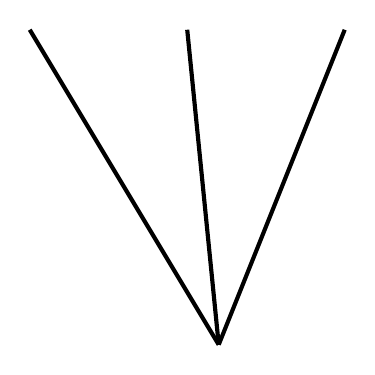
\begin{tikzpicture}

	\draw[line width=1.5pt] (3,0) -- (0.6,4);
	\draw[line width=1.5pt] (3,0) -- (2.6,4);
	\draw[line width=1.5pt] (3,0) -- (4.6,4);

\end{tikzpicture}
\caption{Amoeba architecture.}
\label{amoeba-architecture}
\end{figure*}

\nocite{*}
\bibliographystyle{ieeetr} %plain, ieeetr
\bibliography{Wormref}

\end{document}




